% [1] Guo, Jiaqi, et al. “Towards complex text-to-SQL in the cross-domain database with intermediate representation.” arXiv preprint arXiv:1905.08205 (2019).

\subsection*{IRNet}

\begin{itemize}
    \item In Text2SQL tasks, the Intermediate Representation Network (IRNet) addresses two main challenges.
    \item Among the challenges are mismatches between natural language intents and predicting columns resulting from a more significant number of out-of-domain words.
    \item Instead of synthesizing SQL queries end-to-end, IRNet decomposes natural language into three phases.
    \item Schema linking is performed over a database schema and a question during the first phase.
    \item IRNet uses SemQL to bridge the gap between SQL and natural language.
    \item It includes a Natural Language (NL) encoder, a Schema Encoder, and a Decoder.
\end{itemize}

\begin{figure}[htb]
    \centering
    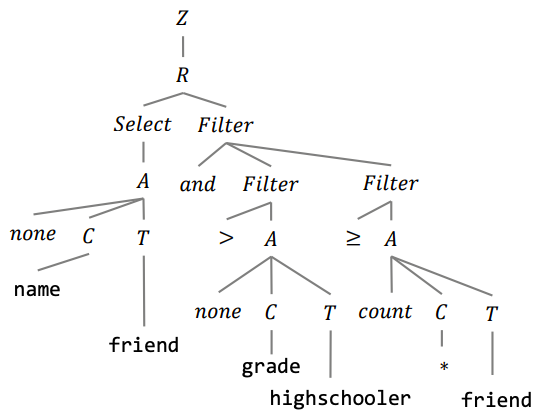
\includegraphics[width=0.8\textwidth]{pics/IRNet/illustrative_SemSQL}
    \caption{An illustrative example of SemSQL from [1]}
    \label{fig:illustrative_SemSQL}
\end{figure}

\begin{figure}[htb]
    \centering
    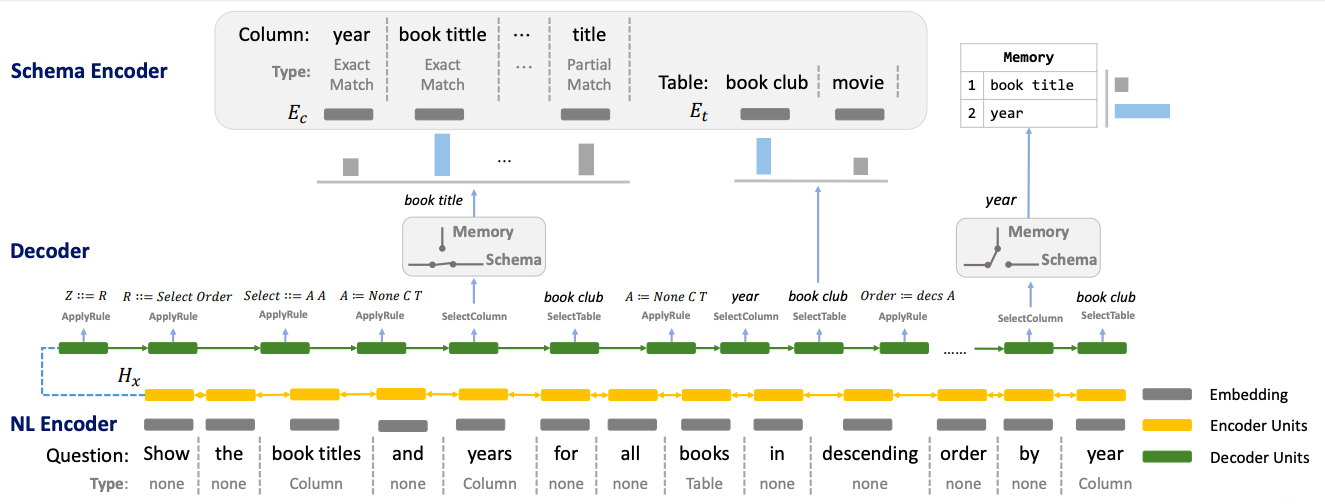
\includegraphics[width=0.8\textwidth]{pics/IRNet/overview}
    \caption{An overview of the neural model proposed in [1]}
    \label{fig:overview}
\end{figure}

\begin{itemize}
    \item The model provides different functions to accomplish Text2SQL tasks.
    \item Natural language is encoded into an embedding vector by the NL encoder. By using a bi-directional LSTM, these embedding vectors are used to construct hidden states.
    \item A schema encoder takes a database schema as input and outputs representations for columns and tables.
    \item Using a context-free grammar, the decoder synthesizes SemQL queries.
    \item On the SPIDER dataset, IRNet performs 46.7\% better than previous benchmark models by 19%.
    \item The accuracy of 54.7\% is achieved by combining IRNet with BERT.
\end{itemize}

\begin{figure}[htb]
    \centering
    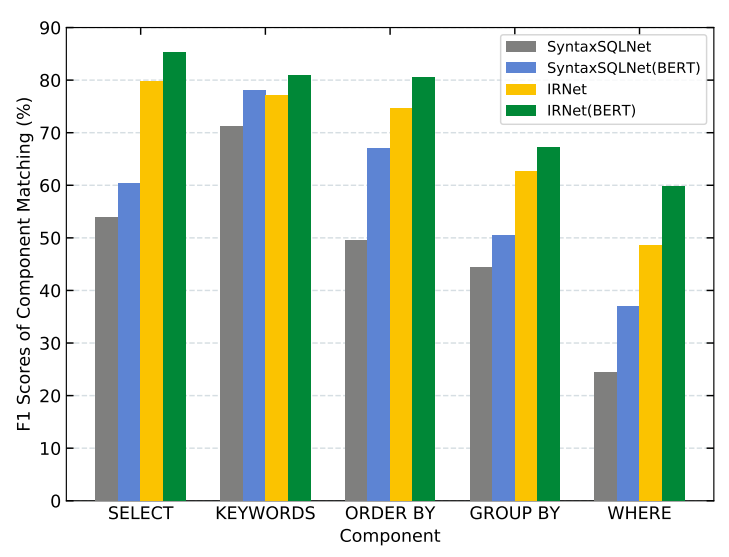
\includegraphics[width=0.8\textwidth]{pics/IRNet/f1}
    \caption{F1 scores of component matching of SyntaxSQLNet, SyntaxSQLNet(BERT), IRNet and IRNet(BERT) on the test set from [1]}
    \label{fig:f1}
\end{figure}
